\section*{Цель работы}
Изучение явления внешнего фотоэффекта; экспериментальное исследование вольт-амперной, световой и спектральной характеристик вакуумного фотоэлемента.

\section*{Приборы и принадлежности}
Модульный учебный комплекс МУК-ОК, в состав которого входят стенд с объектами исследования С3-ОК01, амперметр-вольтметр АВ-1, источник питания ИПС1, соединительные проводники.

\section*{Исследуемые закономерности}
\textit{Внешний фотоэффект} — явление испускания электронов (фотоэлектронов) веществом под действием падающего светового излучения. Регистрируемый с помощью амперметра световой ток является суперпозицией «истинного» фототока $I_\text{ф}$ и темнового тока $I_\text{т}$.
$$ I = I_\text{ф} + I_\text{т} $$

В данной лабораторной работе исследуются следующие основные характеристики фотоэлемента:
\begin{enumerate}
    \item \textit{Вольт-амперная характеристика} — зависимость силы фототока от напряжения между катодом и анодом для выбранных значений падающего светового потока $\Phi$ с определенной длиной волны $\lambda$.
          $$ I_\text{ф} = f(U)|_{\Phi=\text{const}, \lambda=\text{const}} $$
          С увеличением напряжения фототок возрастает и при некотором напряжении $U_A$ достигает насыщения $I_{\text{ф.н}}$, когда все выбитые электроны достигают анода.

    \item \textit{Световая характеристика} — зависимость фототока насыщения $I_{\text{ф.н}}$ от светового потока $\Phi$ при неизменном его спектральном составе.
          $$ I_{\text{ф.н}} = f(\Phi)|_{U=\text{const}, \lambda=\text{const}} $$
          Эта характеристика является линейной (при условии отсутствия объемного заряда).

    \item \textit{Спектральная характеристика} — зависимость фототока насыщения $I_{\text{ф.н}}$ от длины волны $\lambda$ падающего света при неизменной величине светового потока.
          $$ I_{\text{ф.н}} = f(\lambda)|_{\Phi=\text{const}, U=\text{const}} $$
\end{enumerate}

\begin{figure}[H]
    \centering
    \begin{minipage}{0.48\linewidth}
        \centering
        \def\thefigure{6.6}
        \protect\phantomsection
        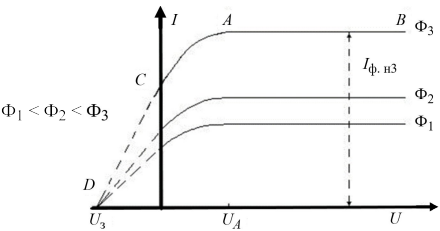
\includegraphics[width=0.9\linewidth]{figs/6-6.png}
        \caption{Вольт-амперные характеристики фотоэлемента}
        \label{fig:va_char}
    \end{minipage}\hfill
    \begin{minipage}{0.48\linewidth}
        \centering
        \def\thefigure{6.7}
        \protect\phantomsection
        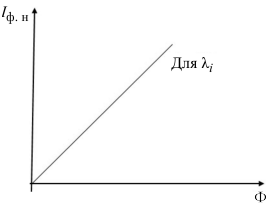
\includegraphics[width=0.9\linewidth]{figs/6-7.png}
        \caption{Световая характеристика вакуумного фотоэлемента}
        \label{fig:light_char}
    \end{minipage}
\end{figure}

\newpage
\centeredsection{\MakeUppercase{Указания по проведению эксперимента}}

\begin{figure}[H]
    \centering
    \begin{minipage}{0.48\linewidth}
        \centering
        \def\thefigure{6.4}
        \protect\phantomsection
        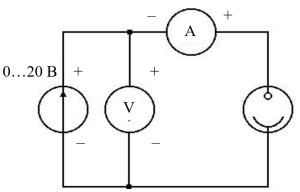
\includegraphics[width=0.9\linewidth]{figs/6-4.png}
        \caption{Электрическая схема экспериментальной установки}
        \label{fig:circuit}
    \end{minipage}\hfill
    \begin{minipage}{0.48\linewidth}
        \centering
        \def\thefigure{6.5}
        \protect\phantomsection
        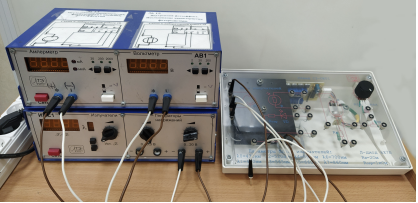
\includegraphics[width=0.9\linewidth]{figs/6-5.png}
        \caption{Модульный учебный комплекс МУК-ОК}
        \label{fig:setup}
    \end{minipage}
\end{figure}

\begin{enumerate}
    \item \textbf{Собрать электрическую схему} с помощью соединительных проводников на стенде С3-ОК01 (см. \cref{fig:circuit}).

    \item \textbf{Настроить приборы.} На блоке АВ-1 выбрать режим измерения вольтметра ($0...20$ В) и амперметра (– $20$ мкА).

    \item \textbf{Снять темновую характеристику} $I_\text{т} = f(U)$ при относительном световом потоке $\Phi \sim J/J_0 = 0.1$ и длине волны $\lambda_4$. Измерения проводить в диапазоне напряжений $U = 0...20$ В с шагом $\Delta U = 1$ В. Результаты занести в \cref{tab:protocol_V-A}.

    \item \textbf{Снять семейство вольт-амперных характеристик} $I=f(U)$ для трех значений светового потока $\Phi$ (например, $(J/J_0)_1=0.3$, $(J/J_0)_2=0.7$, $(J/J_0)_3=1.1$) при длине волны $\lambda_4$. Результаты занести в \cref{tab:protocol_V-A}.

    \item \textbf{Снять спектральную характеристику.} Измерить световой ток $I$ для всех длин волн $\lambda_0 ... \lambda_7$ при фиксированном напряжении насыщения $U_\text{н}$ (например, $20$ В) и постоянном световом потоке (например, $J/J_0=1.1$). Для каждой длины волны измерить темновой ток $I_\text{т}$ (при $J/J_0=0.1$, $U_\text{н}=20$ В). Результаты занести в \cref{tab:protocol_spectral}.
\end{enumerate}

\newpage
\thispagestyle{empty}
\centeredsection{ПРОТОКОЛ НАБЛЮДЕНИЙ}

\begin{table}[H]
    \centering
    \caption{Вольт-амперные характеристики фотоэлемента ($I_\text{ф} = f(U)_{\Phi=\text{const}}$), $\lambda = \lambda_4$.}
    \label{tab:protocol_V-A}
    \begin{tabularx}{\linewidth}{|C||C||C|C||C|C||C|C|}
        \hline
        % Заголовок, занимающий 8 столбцов
        \multirow{2}{*}{$U$, В} & \multirow{2}{*}{$I_\text{т}$} & \multicolumn{2}{c||}{$(J/J_0)_1 = \rule{1.5cm}{0.4pt}$} & \multicolumn{2}{c||}{$(J/J_0)_2 = \rule{1.5cm}{0.4pt}$} & \multicolumn{2}{c||}{$(J/J_0)_3 = \rule{1.5cm}{0.4pt}$}                                     \\
        \cline{3-8}
        % Вторая строка заголовка для 6 столбцов (первые два заняты \multirow)
                                &                               & $I$                                                     & $I_\text{ф}$                                            & $I$                                                     & $I_\text{ф}$ & $I$ & $I_\text{ф}$ \\
        \hline \hline
        % Строки данных, каждая содержит 8 ячеек (7 символов '&')
        0                       &                               &                                                         &                                                         &                                                         &              &     &              \\ \hline
        1                       &                               &                                                         &                                                         &                                                         &              &     &              \\ \hline
        2                       &                               &                                                         &                                                         &                                                         &              &     &              \\ \hline
        3                       &                               &                                                         &                                                         &                                                         &              &     &              \\ \hline
        4                       &                               &                                                         &                                                         &                                                         &              &     &              \\ \hline
        5                       &                               &                                                         &                                                         &                                                         &              &     &              \\ \hline
        6                       &                               &                                                         &                                                         &                                                         &              &     &              \\ \hline
        7                       &                               &                                                         &                                                         &                                                         &              &     &              \\ \hline
        8                       &                               &                                                         &                                                         &                                                         &              &     &              \\ \hline
        9                       &                               &                                                         &                                                         &                                                         &              &     &              \\ \hline
        10                      &                               &                                                         &                                                         &                                                         &              &     &              \\ \hline
        11                      &                               &                                                         &                                                         &                                                         &              &     &              \\ \hline
        12                      &                               &                                                         &                                                         &                                                         &              &     &              \\ \hline
        13                      &                               &                                                         &                                                         &                                                         &              &     &              \\ \hline
        14                      &                               &                                                         &                                                         &                                                         &              &     &              \\ \hline
        15                      &                               &                                                         &                                                         &                                                         &              &     &              \\ \hline
        16                      &                               &                                                         &                                                         &                                                         &              &     &              \\ \hline
        17                      &                               &                                                         &                                                         &                                                         &              &     &              \\ \hline
        18                      &                               &                                                         &                                                         &                                                         &              &     &              \\ \hline
        19                      &                               &                                                         &                                                         &                                                         &              &     &              \\ \hline
        20                      &                               &                                                         &                                                         &                                                         &              &     &              \\ \hline
    \end{tabularx}
\end{table}

\vfill
\noindent
Рахметов А. Р., гр. 4494 ~~\hrulefill~~ «\rule{1cm}{0.4pt}» \rule{3cm}{0.4pt} 20\rule{0.75cm}{0.4pt} г.

\newpage
\thispagestyle{empty}
\centeredsection{ПРОДОЛЖЕНИЕ ПРОТОКОЛА НАБЛЮДЕНИЙ}
\begin{table}[H]
    \centering
    \caption{Спектральная характеристика фотоэлемента ($I_\text{ф.н} = f(\lambda)_{\Phi=\text{const},~U=\text{const}}$), $J/J_0 = \rule{1.5cm}{0.4pt}$, $U = \rule{1.5cm}{0.4pt}$ В.}
    \label{tab:protocol_spectral}
    \begin{tabularx}{\linewidth}{|c|*{8}{C|}}
        \hline
        $\lambda$    & 430 & 470 & 520 & 565 & 590 & 660 & 700 & 860 \\
        \hline \hline
        $I$          &     &     &     &     &     &     &     &     \\
        \hline
        $I_\text{т}$ &     &     &     &     &     &     &     &     \\
        \hline
        $I_\text{ф}$ &     &     &     &     &     &     &     &     \\
        \hline
    \end{tabularx}
\end{table}

\textit{Примечание: } $[\lambda_\forall] = [\text{нм}]$; \hfill $[I_\forall] = [\text{мкА}]$; \hfill $I_\text{ф} = I - I_\text{т}$

\vfill
\noindent
Рахметов А. Р., гр. 4494 ~~\hrulefill~~ «\rule{1cm}{0.4pt}» \rule{3cm}{0.4pt} 20\rule{0.75cm}{0.4pt} г.